\section{Auswertung}
\label{sec:Auswertung}

Im Folgenden wird die Fehlerfortpflanzung und Standardabweichung mittels der Python Bibliothek uncertainties \cite{uncertainties}
berechnet.

\subsection{Filterkurve des Selektiv-Verstärkers}

In diesem Versuchsteil soll die Filterkurve des verwendeten Selektiv-Verstärkers bei 
einer Güte von $Q=20$ untersucht werden.\\
Es werden bei immer höheren Frequenzen des Sinusgenerators eingestellt und die resultierenden
Spannungen im Wechselstrom-Milli-Voltmeters abgelesen. Die aufgenommenen Werte sind in 
\autoref{tab:Filterkurve} zu sehen. Es wurde eine Verstärkung von x10 verwendet. Die eigentlich
resultierenden Spannung sind also nur 0,1x so groß wie die in der Tabelle angegebenen.\\

\begin{table}
  \centering
  \caption{Gemessene Ausgangsspannungen in Abhängigkeit der Frequenz des Sinusgenerators.}
  \label{tab:Filterkurve}
  \begin{tabular}{c | c || c | c}
    \toprule
    Frequenz $f$ / kHz & Ausgangsspannung $U_{\mathrm{A}}$ / V & Frequenz $f$ / kHz & Ausgangsspannung $U_{\mathrm{A}}$ / V \\
    \hline
    10,17 &  0,16  &  22,10 &  8,50 \\
    13,81 &  0,36  &  22,40 &  7,00 \\
    18,23 &  0,90  &  23,10 &  2,90 \\
    19,40 &  1,50  &  24,40 &  1,00 \\
    20,10 &  2,40  &  26,10 &  0,50 \\
    21,00 &  5,20  &  30,80 &  0,30 \\
    21,50 &  8,30  & & \\
    \midrule
    \bottomrule
  \end{tabular}
\end{table}

Die aufgenommenen Messwertpaare werden nun in einem Diagramm gegeneinander geplotted. Die 
enstehende Graphik zeigt wie zu erwarten eine Glockenkurve nach der Gleichung
\begin{equation*}
  U(f) = e^{-a(f-\nu_0)^2}.
\end{equation*}
Die Graphik mitsamt der mit Python gefiteten Glockenkurve ist in \autoref{Abb:Filterkurve} zu sehen.\\
Damit die Graphik besser zu lesen ist, werden die Messwerte der Spannung relativ zur 
maximal gemessenen Spannung $U_{\mathrm{max}} = 8,5 \si{\volt}$ geplotted. Der in der Formel
der Glockenkurve verwendeten Parameter $\nu_0$ gibt die Verschiebung der Glockenkurve an.
Mittels der Python library scipy wurde ein Wert von $\nu_0 = (21,79 \pm 0,07) \, \si{\kilo\hertz} $
berechnet. Für den Parameter $a$ gibt Python den Wert 
$a = (0,52 \pm 0,07 ) \, \si{\per\square\kilo\hertz}$.\\
\begin{figure}
  \centering
  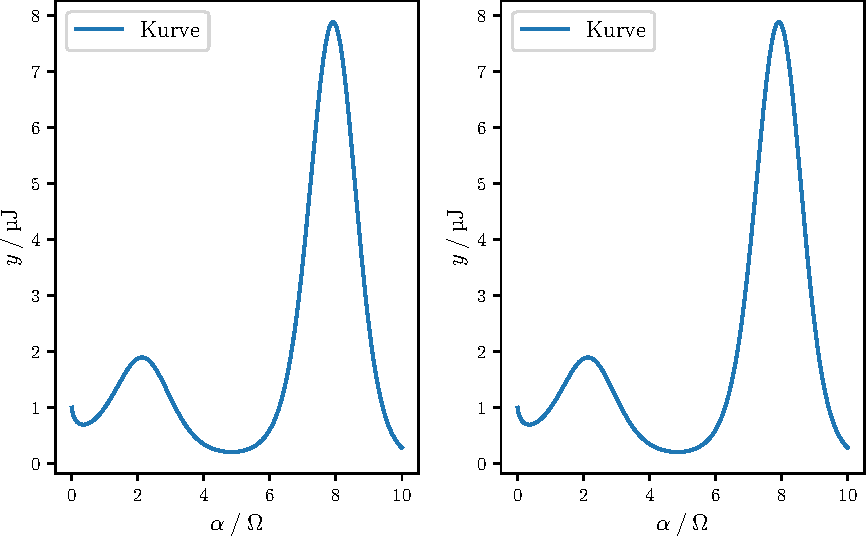
\includegraphics[width=1\textwidth]{build/plot.pdf}
  \caption{Filterkurve des Selektiv-Verstärkers.}
  \label{Abb:Filterkurve}
\end{figure}
Die Frequenzen $\nu_{-}$ und $\nu_{+}$ sind die Schnittpunkte des Fits mit der Geraden
$f(x) = \frac{1}{\sqrt{2}}$. Die Schnittstellen wurden mittels eines Grafischen Taschenrechners
ermittelt und ergaben die Werte $\nu_{-} = 20,97 \, \si{\kilo\hertz}$ und $\nu_{+} = 22,60 \, \si{\kilo\hertz}$.\\
Mit \autoref{eqn:Guete} lässt sich nun die Güte bestimmen. Mit Gaußscher Fehlerfortpflanzung ergibt sich
für die zu untersuchende Filterkurve $Q = (13,37 \pm 0,04)$.\\
Die relative Abweichung zu unserem Theoriewert $Q^* = 20$ lässt sich mit der Gleichung
\begin{equation*}
    \Delta_{\mathrm{rel}}(Q) = \frac{|Q^* - Q|}{Q^*}
\end{equation*}
berechnen. Einsetzen ergibt den Wert $\Delta Q = 33,15 \%$.\\

\subsection{Bestimmung der Suszeptibilitäten drei seltener Erden}

Zur experimentellen Bestimmung der Suszeptibilitäten von Neodym(III)oxid, 
Gadolinium(III)oxid und Dysprosium(III)oxid werden zwei Methoden verwendet. 
Bei einer Methode macht man sich die gemessenen Spannungen vor und 
nach dem Abgleichen zur Gute, hier wird \autoref{eqn:chiSp} verwendet. Die zweite Methode
bedient sich dem Unterschied der Widerstände. Hier wird \autoref{eqn:chiWd} genutzt.\\
Für beide Gleichungen wird die Querschnittsfläche der Proben benötigt.
Hierzu werden die Proben vermessen und die Querschnittsfläche gemäß
\begin{equation*}
  Q = \frac{m}{l \cdot \rho}
\end{equation*}
ausgerechnet. $m$ ist die Masse der Probe, $\rho$ die Dichte und $l$ die Länge.
Die originalen Messdaten lassen sich dem Anhang entnehmen. Die Querschnittsflächen
sind in \autoref{tab:Querschnitt} zu finden.

\begin{table}
  \centering
  \caption{Ausgerechneten Querschnittsflächen der Proben.}
  \label{tab:Querschnitt}
  \begin{tabular}{c | c | c }
    \toprule
    $Q_{\mathrm{Nd}}$ / $\si{\square\milli\meter}$ & $Q_{\mathrm{Gd}}$ / $\si{\square\milli\meter}$ & $Q_{\mathrm{Dy}}$ / $\si{\square\milli\meter}$ \\
    \hline
    6,83 & 9,12 & 12,13 \\
    \midrule
    \bottomrule
  \end{tabular}
\end{table}

Der Spulenquerschnitt ist gegeben durch $F = 86,6 \, \si{\square\milli\meter}$, der feste
Widerstand der Schaltung mit $R_3 = 998\,  \si{\ohm}$ und $U_{\mathrm{Sp}}= 8,5 \, \si{\volt}$.
Die nun zur Berechnung fehlenden Größen
$U_{\mathrm{Br}}$ und $\Delta R$ sind bei jeder Messung unterschiedlich
und lassen sich ebenfalls dem Anhang entnehmen. Da pro Probe jeweils drei Messungen 
durchgeführt werden, wird im Anschluss der Mittelwert der Ergebnisse bestimmt. Die Ergebnisse
lassen sich der \autoref{tab:Widerstand} und \autoref{tab:Spannung} entnehmen.\\

\begin{table}
  \centering
  \caption{Experimentell berechnete Suszeptibilitäten aus den Widerständen.}
  \label{tab:Widerstand}
  \begin{tabular}{c || c | c | c || c }
    \toprule
    Probenname & $\chi_1$ & $\chi_2$ & $\chi_3$ & $\overline{\chi}_{\mathrm{exp}}$ \\
    \hline
    $\mathrm{Nd}_2 \mathrm{O}_3$ & 0,0042 & 0,0031 & 0,0028 & 0,0033 $\pm$ 0,0006 \\
    $\mathrm{Gd}_2 \mathrm{O}_3$ & 0,0131 & 0,0131 & 0,0131 & 0,0131 $\pm$ 0 \\
    $\mathrm{Dy}_2 \mathrm{O}_3$ & 0,0236 & 0,0223 & 0,0239 & 0,0233 $\pm$ 0,0007 \\
    \midrule
    \bottomrule
  \end{tabular}
\end{table}

\begin{table}
  \centering
  \caption{Experimentell berechnete Suszeptibilitäten aus den Spannungen.}
  \label{tab:Spannung}
  \begin{tabular}{c || c | c | c || c }
    \toprule
    Probenname & $\chi_1$ & $\chi_2$ & $\chi_3$ & $\overline{\chi}_{\mathrm{exp}}$ \\
    \hline
    $\mathrm{Nd}_2 \mathrm{O}_3$ & 0,0179 & 0,0209 & 0,0194 & 0,0194 $\pm$ 0,0012 \\
    $\mathrm{Gd}_2 \mathrm{O}_3$ & 0,0067 & 0,0067 & 0,0068 & 0,0067 $\pm$ 0 \\
    $\mathrm{Dy}_2 \mathrm{O}_3$ & 0,0369 & 0,0419 & 0,0504 & 0,0430 $\pm$ 0,006 \\
    \midrule
    \bottomrule
  \end{tabular}
\end{table}

Die Theoriewerte der Suszeptibilitäten der Proben werden durch \autoref{eqn:chi} berechnet. Dafür sind
die Quantenzahl J, L und S, die Konstanten $\mu_0$, $\mu_{\mathrm{B}}$ 
und $k_{\mathrm{B}}$, der Landé-Faktor $g_{\mathrm{J}}$, die Anzahl der Momente pro 
Volumeneinheit $N$ und die Temperatur $T$ nötig.\\
Die Quantenzahlen J, L und S werden im Internet nachgeguckt und sind für Neodym(III)oxid 
J = 4.5, L = 6 und S = 1.5 \cite{Nd}, für Gadolinium(III)oxid J = 3.5, L = 0 und S = 3,5 
und für das Dysprosium(III)oxid J = 7.5, L = 5 und S = 2.5 \cite{DyGd}.\\
Die Anzahl der Momente der Volumeneinheit berechnet sich zu $N = \frac{2 N_{\mathrm{A}} \rho }{M}$,
wobei $N_{\mathrm{A}}$ die Avogadro-Konstante und $M$ die molare Masse des Moleküls ist.\\
für die Temperatur wird die Zimmertemperatur mit $T = 293,15 \, \si{\kelvin}$ angenommen.\\
Die Werte werden ausgerechnet und in \autoref{tab:Theorie} dargestellt.

\begin{table}
  \centering
  \caption{Theoretisch berechnete Suszeptibilitäten.}
  \label{tab:Theorie}
  \begin{tabular}{c || c }
    \toprule
    Probenname & $\chi_{\mathrm{theo}}$ \\
    \hline
    $\mathrm{Nd}_2 \mathrm{O}_3$ & 0,0030 \\
    $\mathrm{Gd}_2 \mathrm{O}_3$ & 0,0138 \\
    $\mathrm{Dy}_2 \mathrm{O}_3$ & 0,0254 \\
    \midrule
    \bottomrule
  \end{tabular}
\end{table}

